\documentclass[11pt]{article}

%%% PAGE DIMENSIONS
\usepackage{geometry} % to change the page dimensions
\geometry{a4paper, left=30mm, right=40mm, top=35mm, bottom=25mm} 

%%% PACKAGES
\usepackage{threeparttable}
\usepackage[utf8]{inputenc}
\usepackage{rotating} 
\usepackage{setspace}
\usepackage{subfigure} % pictures (subpictures), tables (subtables)
\usepackage{url} % make url visible
\usepackage{tabularx} % fits the width of a table to width of the text
\usepackage{acronym} % list of abbrevations
\usepackage{amsmath}
\usepackage{amssymb}
\usepackage[german, ngerman, english]{babel}
\usepackage[T1]{fontenc}
\usepackage{booktabs} % for much better looking tables
\usepackage{epstopdf} 
\usepackage[T1]{fontenc}
%\usepackage{natbib} % implements both author-year and numbered references
\usepackage{fancyhdr}

\usepackage[backend = biber, sorting = none]{biblatex}
\usepackage{csquotes}
\addbibresource{references.bib}
\usepackage{hyperref}
\hypersetup{hidelinks}
\usepackage[all]{nowidow}
\counterwithin{figure}{section}
\numberwithin{equation}{section}
\usepackage{textgreek}
\usepackage{makecell}


%%% ToC (table of contents) 
\usepackage[nottoc]{tocbibind} % Put the bibliography in the ToC
\usepackage[titles,subfigure]{tocloft} 
\renewcommand{\cftsecfont}{\rmfamily\mdseries\upshape}
\renewcommand{\cftsecpagefont}{\rmfamily\mdseries\upshape}

%%% END Article customizations

\begin{document}
	
	\parindent 0pt
	
	\pagenumbering{Roman}

	%%% Cover sheet 
	\thispagestyle{empty}


\begin{minipage}{0.825\textwidth}
	\vspace{20pt}
	Augsburg University\\
	Mathematisch-Naturwissenschaftlich-Technische Fakultät\\
	Experimentalphysik I - Institut für Physik\\
	Prof. Dr. Ferdinand Haider\\
\end{minipage}
\begin{minipage}{0.175\textwidth}
	%\hspace*{50}
	
\includegraphics[width=\textwidth]{pictures/Logo_Uni.eps}
\end{minipage}

\vspace{120pt}

\begin{center}
\huge \textbf{Laboratory Report}\\

\vspace{120pt}

\Large Method Course: Electron Microscopy\\
\Large Summer Term 2023
\end{center}

\vspace{80pt}

\normalsize
\begin{tabbing}
Supervised by: \qquad \= Dr.rer.nat. Aladin Ullrich\\
\>\= David Stein\\
\>\= Johannes Berlin\\
\> \\

Submitted by: \>[Vorname1, Name1] [Matrikelnummer1] [Studienfach, Semester]\\
\>[Vorname2, Name2] [Matrikelnummer2] [Studienfach, Semester] \\
\>[Vorname3, Name3] [Matrikelnummer3] [Studienfach, Semester]\\
\>[Vorname4, Name4] [Matrikelnummer4] [Studienfach, Semester]\\
\>[Vorname5, Name5] [Matrikelnummer5] [Studienfach, Semester]\\
\> \\

Submission date: \> 14.08.2023

\end{tabbing}
	\clearpage

	\begin{spacing}{1.5}
		
		%%% abstract
		\include{abstract}
		\clearpage
		
		%%% table of contents
		\tableofcontents
		\clearpage

		%%% List of abbrevations
		\section*{List of abbreviations}




\begin{acronym}[ABSTAND]

\acro{SEM}{Scanning-Electron-Microscope}\\
\acro{TEM}{Transmission-Electron-Microscope}\\


\end{acronym}

		
		%%%"List of abbrevations" in ToC
		\addcontentsline{toc}{section}{List of Abbreviations}%
		
		\clearpage
		
		\pagenumbering{arabic}   
		
		%%%%%%%%%%%%%%%%%%%Beginn

        %%% for document: fancy pagestyle
        \pagestyle{fancy}
        \lhead{}
        \chead{}
        \rhead{\leftmark}
        \lfoot{}
        \cfoot{\thepage}
        \rfoot{}
		\setlength{\headheight}{14.00pt}
  
		\section{Introduction to Electron Microscopy}
\label{sec: introduction}

The investigation of the structure of a material is necessary with regard to many possible reasons and thus the field of material testing is extensive. In the research of materials science and engineering, there is a need of investigation the material in order to determine the relationship of the structure and the properties. The knowledge about the relationship of structure and properties enables the scientists to tune the properties of a material within their production or in further processes. In material testing one can distinguish chemical analysis, examination of structures and defects, destructive and non-destructive testing. Considering this classification of material testing methods, microscopy enables the examination of structures and defects as well as chemical analysis \cite[p.497]{Weißbach_Dahms_Jaroschek_2015}.

\subsection{Magnification and Spatial Resolution}

Microscopes are optical devices with magnification factors bigger than one. If a structure is too small for the observation with the unaided human eye, microscopes are needed to resolve the object by magnifying the object diameter at the object plane to the object resolution of the human eye. The object resolution of an human eye is typically 75\textmu m \cite[p.5]{EGERTON_2016}.\\

The reasonable magnification of an object is limited by the spatial resolution, which describes the minimal size of an object that still need to be clearly distinguished from an adjacent and similar object. The spatial resolution depends on the diffraction of the light or electrons. For the explanation of diffraction, one needs to describe light and electrons as waves. In an example in figure \ref{fig: DiffractionOfLigth}, parallel light of a certain wavelength \textlambda{} strikes an opaque screen with a circular aperture of radius a. A white display screen is then illuminated and shows a circular pattern with diffuse edges, called Airy disk. Light from a secondary source arrives at certain angle \straighttheta{} and forms a displaced Airy disk. According to the Rayleigh criterion the resolution of the two sources can only be achieved, if the displaced Airy maximum coincides with the first Airy minimum of the initial source. From diffraction theory, one can derive the smallest distance between two distinguishable specimen points leading to equation \ref{eqn: diffraction_theory} \cite[p.3]{EGERTON_2016}.

\begin{equation}
    \Delta x \approx 0.61 \cdot \frac{\lambda}{a}
    \label{eqn: diffraction_theory}
\end{equation}

This approximation holds only for \textlambda{} $\ll$ a due to the application of a small-angle approximation within the derivation: $sin\theta \approx tan\theta$. As the diffraction occurs if the wavelength of the light is in equal size or smaller than the circular aperture, one can improve the resolution by applying smaller wavelengths than the size of the circular aperture \cite{LectureEM-Haider}.\\ dd \ref

\begin{figure}[!ht]
	\centering
	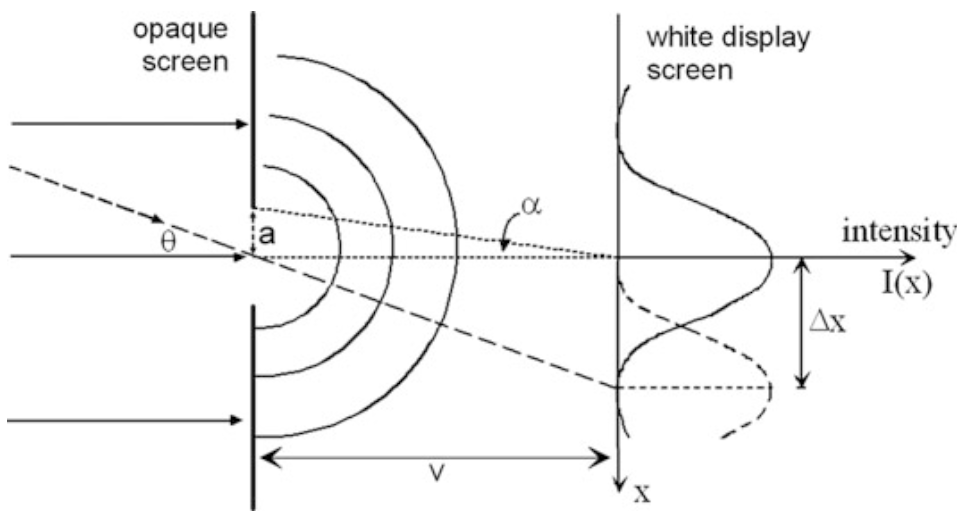
\includegraphics[width=12cm]{pictures/pictures_ch1/Diffraction.png}
	\caption{Diffraction of waves \cite[p.3]{EGERTON_2016}}
	\label{fig: DiffractionOfLigth}
\end{figure}

\subsection{Different Forms of Microscopes}

The first light microscopes were developed in the 1600s using one-lens devices to observe bacteria within cells of animal tissue. Further developments lead to compound microscopes with at least two lenses. One lens is placed close to the eye (eyepiece) and one is placed close to the object (objective). Theoretically one could increase the magnification indefinitely by using higher number of lenses, but this magnification is then limited by the resolution. The best-possible resolution that can be achieved using a light microscope for light in the middle of the visible spectrum (\textlambda{}= 0.5\textmu m) is about 0.3\textmu m. If the object resolution of the human eye is divided by the resolution of 0.3\textmu m, the required magnification factor of 250 can be estimated. A larger magnification wouldn't improve the sharpness of the image \cite[p.6]{EGERTON_2016}. Nevertheless, light microscopes can reach magnification factors of 1000 \cite[p.550]{Weißbach_Dahms_Jaroschek_2015}. They are widely used in two forms: either as biological microscopes or as metallurgical microscopes. With biological microscopes, optically transparent specimens can be investigated to reveal organelles within biological cells. Metallurgical light microscopes are used for the investigation of bulk materials like metals. The image is then formed by the reflected light and can e.g. reveal grain shape and size of an alloy.\\

If the observable structure is too small for the investigation with light, electron beams have to be used instead of light to resolve the structure. Visible light has a wavelength of 400-700nm \cite[p.4]{Zwinkels2014}, whereas the wavelength of electrons with certain acceleration voltages can be much shorter. Considering the wave-particle duality using the De-Broglie wavelength of an electron given by equation \ref{eqn: de_broglie}, the wavelength of an electron accelerated by acceleration voltage $U_{A}$ can be calculated. 

\begin{equation}
    \lambda_{DB} = \frac{h}{p_{e}} = \frac{h}{m_{e} \cdot v_{e}} = 
    \frac{h}{\sqrt{2 \cdot m_{e} \cdot E_{kin}}} =
    \frac{h}{\sqrt{2 \cdot m_{e} \cdot e \cdot U_{A}}}
\label{eqn: de_broglie}
\end{equation}
where:
\begin{tabbing}
\hspace{2em} \= \hspace{3em} \=  = \= \kill
\> $\lambda_{DB}$ \> = De-Broglie wavelength of an electron\\
\> $h$ \> = Planck constant ($6.626 \cdot 10^{-34} Js$)\\
\> $p_{e}$ \> = Momentum of an electron\\
\> $m_{e}$ \> = Electron-mass ($9.109 \cdot 10^{-31}kg$)\\
\> $v_{e}$ \> = Electron-velocity\\
\> $e$ \> = Charge of an electron ($1.602 \cdot 10^{-19}As$)\\
\> $E_{kin}$ \> = Kinetic energy of an electron accelerated by $U_{A}$\\
\> $U_{A}$ \> = Acceleration voltage\\
\end{tabbing}

Equation \ref{eqn: de_broglie_ex} gives an example of an electron accelerated by 30kV resulting in a wavelength of approximately 0.007nm. With this wavelength, the electrons are not diffracted by the atoms of the sample surface and thus can penetrate into the material by several micrometers \cite[p.10]{EGERTON_2016}.

\begin{equation}
    \lambda_{DB}(E_{kin}=30kV) = \frac{h}{\sqrt{2 \cdot m_{e} \cdot e \cdot U_{A}}} = 7.1 \cdot 10^{-12}m \approx 0.007nm
\label{eqn: de_broglie_ex}
\end{equation}

Modern \acfp{TEM} use electron-accelerating voltages from 60 to 300kV, resulting in energies and thus wavelengths that enable scientists to resolve structures on atomic scale. The electrons are then diffracted by atomic planes in the material and therefore a transmission diffraction pattern of the electrons that have passed through the specimen can be formed. Hence, the application of \acp{TEM} is based on the preparation of thin samples which can be permeated by electrons. If the electrons are focused with their short wavelengths after passing the thin sample, an image with a very high resolution of even below 0.2nm can be formed \cite[p.10]{EGERTON_2016}. The \acp{TEM} are hence useful for the examination of atomic structures and crystalline defects in materials.\\

\acfp{SEM} usually accelerate the electrons with voltages up to 30kV. Hence, their resolution is not as good as the resolution of a \ac{TEM}, but still superior to the one of light microscopes. The advantage of \acp{SEM} is that also bulk materials can be investigated by analysis of electron-solid interaction signals that will be discussed more detailed in section \ref{sec: SEM}. The image formation is based on the raster scanning principle, meaning that the electron beam is lead over the specimen surface in a rectangular area and in two perpendicular directions. The final image is then produced by the software of the \ac{SEM}. Compared with the simultaneous image generation of an \ac{TEM}, a \acp{SEM} hence generates the image serially. Modern \acp{SEM} provide image resolutions between 1 and 10nm. Additionaly, they provide a large depth of focus which results from the fact that electrons in the \ac{SEM} move close to the optic axis \cite[p.16]{EGERTON_2016}.\\

\begin{table}[!ht]
\centering
\begin{tabular}{|c|c|c|c|} 
 \hline
 Property & Light Microscope & \makecell{SEM} & \makecell{TEM}\\  
 \hline 
 \makecell{Magnification\\factor} & up to 1000 & up to 200000 & up to 1000000\\ \hline
 \makecell{Spatial resolution} & 0.3\textmu m & 1-10nm &  $\leq$ 0.2nm\\ \hline
 \makecell{Acceleration\\voltage range} & & $\leq$ 30kV & 60-300kV\\ \hline
 Structures & \makecell{grains\\biological organelles} & \makecell{microstructures} & \makecell{atomic planes,\\crystalline defects}\\ 
 \hline
\end{tabular}
\caption{Properties of different microscopes b.o. \cite[p.550]{Weißbach_Dahms_Jaroschek_2015} and \cite[p.9-16]{EGERTON_2016}}
\label{table: microscopes}
\end{table}

Table \ref{table: microscopes} summarizes the characteristics of the microscopes described above. Within this method course, the physical principles of scanning electron microscopy and transmission electron microscopy are discussed in the lecture and validated in practical applications in the laboratory. The aim of the course is further to enable the students to operate \acp{SEM} and \acp{TEM} on a basic level and characterize materials using different electron microscopy techniques. Therefore, this laboratory report consists of a theoretical description of the microscopes, detectors and operation modes and of the assessment of the practical examples performed in the laboratory afterwards.

\newpage
    
		
		
		\section{Concepts of Electron Optics}
\label{sec: electron_optics}

Before going into detailed descriptions of different electron microscopes, it is useful to summarize general concepts of electron optics. This involves the definition of properties of an ideal image, principles in imaging with electrons and defects and their corrections of electron lenses.

\subsection{Properties of an Ideal Image}

According to James Clark Maxwell, the quality of an image can be defined by fulfilling three requirements that ensure close resemblance of the image to the corresponding object. These requirements can be taken for characterization of image defects as well for a description for negative examples as follows.\\

The first requirement is that each point in an image, there should be an equivalent point in the object. This requirement is determined by the properties of the optical system. Negative examples would be incorrect focus strength leading to an image formed out of focus. Even at optimal focus strength, aberrations of the lenses could still lead to blurred images with a loss of spatial resolution. Maxwell's second requirement states that the object and the image should exhibit similar geometry meaning that they should show similar patterns of points. Hence, the requirements demands similar geometrical sense, but different orientation or inversion is allowed. Real images can show distortions that correlate to a positional variation of the magnification. Figure \ref{fig: commonDistortions} shows three common distraction types: pincushion distortion (a), barrel distortion (b) and spiral distortion. Pincushion distortion results by an increasing magnification with radial distance from the optic axis, whereas barrel distortion corresponds to a decreasing magnification away from the optic axis. Spiral distortion results, if rotation of the image depends on the distance of the point from the optic axis. The third requirement demands that images are typically of two dimensions and occupy in a flat plane. Hence, if the object is planar and perpendicular to the optic axis, so is the image. If the focusing power of a lens depends on the object distance to the optic axis, the optic systems shows curvature of field \cite[p.27 f.]{EGERTON_2016}. 

\begin{figure}[!ht]
	\centering
	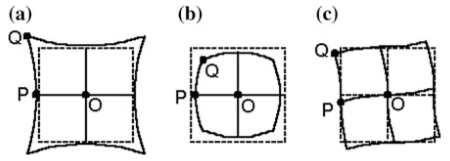
\includegraphics[width=10cm]{pictures/pictures_ch2/Distortions.png}
	\caption{Common types of distortions \cite[p.29]{EGERTON_2016}}
	\label{fig: commonDistortions}
\end{figure}

\subsection{Electron Sources}
\subsection{Electron Lenses, Defects and Correction}

In order to focus a light beam, light optics use convex lenses. Electron optics is based on similar principles of image formation. The equivalent of an convex lens in light optics are either electrostatic or magnetic lenses in electron optics. using either electrostatic or magnetic fields to deflect the electron's trajectories.\\

The simple arrangement of an electrostatic lens could be described as a circular conducting electrode with a circular hole for the optic axis. The circular electrode is further connected to a negative voltage and hence electrons passing the hole with a trajectory not lying on the optic axis are repelled by the non-uniform electric field. The deflection angle hence depends on the displacement from the optic axis. For the purpose of focusing, the formation of a point image can be expected out of the electrons originating from point source as pictured in figure \ref{fig: unipotentialLens}. In particular, the electrostatic lens in figure \ref{fig: unipotentialLens} is known as unipotential lens or einzel lens. Unipotential lenses consist of additional circular electrodes placed before and after the the central electrode to limit the extent of the electric field. This ensures that the electrons leave with the same potential as they enter with. The electrostatic fields further show cylindrical symmetry, hence the focusing force depends only on the radial distance from the optic axis. and is independent of the azimuthal direction around the axis \cite[p.33]{EGERTON_2016}.\\



\begin{figure}[!ht]
	\centering
	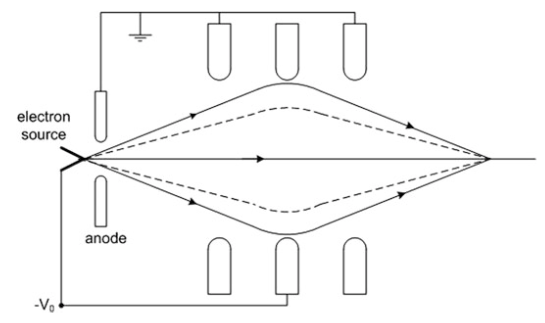
\includegraphics[width=10cm]{pictures/pictures_ch2/UnipotentialLens.png}
	\caption{Unipotential, electrostatic lens \cite[p.33]{EGERTON_2016}}
	\label{fig: unipotentialLens}
\end{figure}

\newpage        
  
		\section{The Scanning-Electron-Microscopy}
\label{sec: SEM}
 
Welcome to SEM.

\newpage
		

        \section{The Transmission-Electron-Microscope}
\label{sec: TEM}
xy
 
\newpage
		

        %% stop fancy pagestyle for rest of document
       \pagestyle{plain}

  
        \printbibliography
        \clearpage

        %%% list of figures
        \listoffigures
        \clearpage

        %%% list of tables
        \listoftables
        \clearpage
		
		\section*{Appendix}
\addcontentsline{toc}{section}{Appendix}
\label{sec:anhang} % ANHANG A

\setcounter{figure}{0}
\renewcommand{\thefigure}{A.\arabic{figure}}

\setcounter{table}{0}
\renewcommand{\thetable}{A.\arabic{table}}



		\clearpage
		
		%% declaration of an oath
        \input{declaration}
		\clearpage
		
	\end{spacing}
	
	
\end{document}